% Standalone research report. Build with build_report.py; data snapshots are included.
\documentclass[11pt,letterpaper]{article}
\usepackage[T1]{fontenc}
\usepackage[utf8]{inputenc}
\usepackage{lmodern,microtype}
\usepackage[margin=0.85in,headheight=15pt]{geometry}
\usepackage{amsmath,amssymb,bm}
\usepackage{graphicx,booktabs,tabularx,longtable,array}
\usepackage[table]{xcolor}
\usepackage{tikz}
\usetikzlibrary{arrows.meta,positioning,fit,backgrounds,calc}
\usepackage[most]{tcolorbox}
\usepackage{enumitem,placeins,fancyhdr}
\usepackage{url}
\usepackage[colorlinks=true,linkcolor=tealblue,citecolor=tealblue,urlcolor=tealblue,breaklinks=true]{hyperref}
\definecolor{tealblue}{HTML}{007C83}
\definecolor{ink}{HTML}{172C3B}
\definecolor{pale}{HTML}{EFF6F7}
\definecolor{warm}{HTML}{CF7B35}
\definecolor{muted}{HTML}{526477}
\hypersetup{pdftitle={Shared Mechanical Policies for Cross-Embodiment Locomotion},pdfsubject={Architecture, experimental evidence, limitations and research directions},pdfauthor={Isaac Lab / Newton research notes}}
\setlength{\parindent}{0pt}
\setlength{\parskip}{0.45em}
\setlength{\emergencystretch}{2em}
\setlist{nosep,leftmargin=1.5em,topsep=0.4em}
\renewcommand{\arraystretch}{1.18}
\newcolumntype{Y}{>{\raggedright\arraybackslash}X}
\newcommand{\R}{\mathbb{R}}
\newcommand{\mech}{\mathcal{M}}
\newcommand{\state}{s}
\newcommand{\policy}{\pi_\theta}
\newcommand{\code}[1]{\texttt{#1}}
\newcommand{\reportdate}{7 October 2026}
\makeatletter
\newcommand{\tableinput}[1]{\@@input #1 }
\makeatother
\newtcolorbox{finding}[1]{colback=pale,colframe=tealblue,boxrule=0.5pt,arc=1mm,title={#1},fonttitle=\bfseries,breakable}
\pagestyle{fancy}
\fancyhf{}
\fancyhead[L]{\small\color{muted}Shared mechanical policies}
\fancyhead[R]{\small\color{muted}Research snapshot / October 2026}
\fancyfoot[C]{\small\thepage}
\renewcommand{\headrulewidth}{0.3pt}
\tikzset{box/.style={draw=tealblue,fill=pale,rounded corners=2pt,align=center,font=\small,minimum height=11mm,inner sep=5pt},arr/.style={-{Latex[length=2mm]},thick,draw=muted}}

\begin{document}
\hypersetup{pageanchor=false}
\begin{titlepage}
\vspace*{14mm}
{\large\color{tealblue}\bfseries ISAAC LAB / NEWTON RESEARCH NOTES\par}
\vspace{12mm}
{\Huge\bfseries\color{ink}Shared Mechanical Policies\par}
\vspace{3mm}
{\LARGE\color{ink}for Cross-Embodiment Locomotion\par}
\vspace{9mm}
{\Large Architecture, experimental evidence,\par limitations, and research directions\par}
\vspace{12mm}
{\large\reportdate\par}
\vfill
\begin{finding}{Current conclusion}
A single mechanical-token attention policy reproduces fast locomotion on the
three- and four-leg training robots after specialist distillation. This establishes
source-control capability in the present setup. Frozen transfer tests find slow
motion on five legs and rapid falls on simulated Unitree Go2/A1. A subsequent Go2
specialist learns the task, but solo and mixed-family attention imitation still
fail on Go2. Mechanical understanding, reliable transfer and an original
algorithmic contribution remain research questions.
\end{finding}
\vspace{6mm}
\textbf{Document status.} Consolidated technical report of existing code and saved
experiments. Proposed methods and experiments are labeled explicitly.
The October 7 extensions add frozen target evaluations in
Section~\ref{sec:transfer} and new Go2 specialist/student training in
Section~\ref{sec:go2learning}, all with the existing training seed 42.
No independent training-seed sweep was performed.
The accompanying source package contains the result snapshots,
vector figures, bibliography, and rebuild script.
\end{titlepage}

\pagenumbering{roman}
\hypersetup{pageanchor=true}
\tableofcontents
\clearpage
\pagenumbering{arabic}

\section{Executive assessment}
\label{sec:assessment}

The practical objective is to reuse a controller across mechanical systems with
different numbers of bodies and actuators. The immediate question was more basic:
why did our shared graph and attention policies move much more slowly than
conventional specialist neural networks, even on their training robots?

The latest diagnostic changes the answer. Keeping the actor architecture and
physical inputs intact, specialist imitation produces competent shared source
control. The leading attention checkpoint reaches 5.566 and 5.032\,m/s on the
three- and four-leg robots, with 97.9\% and 100\% time-limit survival. Those speeds
are 98.3\% and 95.8\% of the freshly evaluated teachers. The same attention
architecture trained with PPO from scratch previously reached 1.276 and
2.346\,m/s. The learning procedure therefore matters substantially in this setup.

The subsequent frozen transfer tests in Section~\ref{sec:transfer} expose the
remaining gap: both actors crawl on five-leg Ant and fail to sustain stance on
the effort-controlled Unitree targets. Additional training families and the
control interface need investigation before increasing network size.

The new-family learning experiment in Section~\ref{sec:go2learning} establishes
a competent Go2 MLP reference, but small expert-state imitation error does not
translate to stable student rollouts. This failure also occurs in the Go2-only
fit, so interference with Ants cannot be its sole explanation. The immediate
learning priority is startup and recovery-state coverage, with the existing
architecture and matched extra-fitting controls.

The result supports three decisions:
\begin{enumerate}
\item Retain distilled attention as the working source-control baseline. Keep the
attention-free mechanical graph as a comparison because it also produces fast
gaits, although its survival is lower.
\item Test transfer and mechanical-feature use before another broad architecture
sweep. A generic capacity objection is insufficient to explain the source gap.
\item Frame novelty around a specific, measurable property of mechanical reuse.
Shared graphs, morphology-conditioned attention and specialist distillation all
have close precedents.
\end{enumerate}

\begin{finding}{Preferred research question}
Can one controller respond usefully to real changes in a robot's mechanics,
remain consistent when only the model's coordinate conventions change, and carry
both properties to previously unseen articulated structures?
\end{finding}

This question has practical applications: payload and motor changes, model import
across different conventions, and reduced training effort for new robot
structures. It also gives us falsifiable hypotheses. If direct conditioning and
ordinary canonicalization already solve the problem, an elaborate new network is
unnecessary. If richer mechanics contribute little under the current rich state
observations, that is useful evidence about where the representation matters.

\subsection{Evidence and operating scope}
The experiment snapshot uses one teacher/student training seed and three
evaluation reset seeds. At the user's request, additional independent-seed runs
are outside the current plan; there is no seed-count gate on exploration. The
rollout repetitions describe variation for these trained checkpoints, not the
reliability of retraining the algorithm. Held-out bodies and disjoint demonstration
splits remain essential to the questions being asked.

The current result is a research pilot, not a universal-robot guarantee. Its task
is flat-ground forward progress with effort control and rich simulator
observations. The frozen transfer extension in Section~\ref{sec:transfer} finds
slow five-leg motion and failure on simulated Unitree targets. Those measurements
are completed. Section~\ref{sec:go2learning} also completes the first new-family
learning comparison; further representation experiments remain proposals.

\section{Problem definition and experiment contract}
\label{sec:problem}

\subsection{One policy over a family of mechanical systems}
Let $\mech$ describe a robot's supported rigid-body mechanics: bodies, joints,
actuators, collision geometry and relevant physical parameters. The simulator
evolves a state according to
\begin{equation}
  \state_{t+1}=F_{\mech}(\state_t,u_t),\qquad
  o_t=O_{\mech}(\state_t),\qquad
  a_t=\policy(o_t,\mech).
  \label{eq:system}
\end{equation}
The physical control $u_t$ is obtained by applying the environment's execution
mapping to the actor's raw output $a_t$. In the current effort benchmark,
\begin{equation}
  u_{t,k}=g_k(\mech)\,\operatorname{clip}(a_{t,k},-1,1),
  \label{eq:effort}
\end{equation}
where $g_k$ is the declared gear/action-effort gain. A different robot can have a
different number of actuator entries $k$, while sharing all actor weights.

Three distinct capabilities should be kept separate. \emph{Interface support}
means that a robot can be encoded and produces an appropriately sized action
vector. \emph{Source competence} means that training robots execute the task
well. \emph{Transfer} means that an unseen robot benefits without source retraining
or with less target learning. The first does not imply either of the others.

\subsection{The current Ant benchmark}
The source pair consists of a radial three-leg Ant variant and the canonical
four-leg Ant. The current family has two actuated joints per leg, giving six,
eight or ten effort actions for three-, four- or five-leg bodies. Control is at
60\,Hz. The objective rewards forward progress on flat terrain; it is not a
commanded-speed or commanded-yaw tracking benchmark.

The richer mechanical policy observes body poses and velocities, joint state,
previous raw actions, and incoming foot-link joint wrenches. Those wrenches are
not direct measurements of foot-ground contact force. Availability of all these
signals on physical hardware has not been demonstrated.

The earlier diverse population contains eight prototypes but only two source
topologies. Its variations change scale, torso density, limb density, motor
strength and damping. Appendix~\ref{app:population} lists the actual settings.
The repeatedly inspected five-leg body is development data; it is not an
untouched final test.

\subsection{Performance and accounting}
The saved speed metric is the existing completed-episode progress statistic.
Survival is the fraction of episodes reaching the time limit, averaged over the
evaluation reset runs. Speed must be read together with survival because fast
partial behavior can coexist with instability. A useful source ratio is
\begin{equation}
  \rho_b=\frac{v_{\text{shared},b}}{v_{\text{teacher},b}},
\end{equation}
for body $b$ under the same task and observation/action contract. Near-zero or
negative teacher speeds would make this ratio uninformative. No such issue
arises for the current canonical teachers.

Our engineering source criterion is at least 90\% of each competent teacher's
speed, at least 95\% survival, and no more than a two-percentage-point survival
loss relative to that teacher. These are operating criteria, not optimality
theorems. Teacher training, demonstration collection, student optimization and
evaluation must be accounted for separately; the imitation study is not an
equal-cost comparison to PPO from scratch.

\section{Mechanical representation}
\label{sec:representation}

\subsection{Typed entities and physical relations}
The exporter reads supported attributes from the finalized Newton model and
builds a typed graph. Bodies, joints, DOFs and collision shapes are all explicit
entities. Keeping these separate allows an unactuated body or collision shape to
contribute information without requiring an action output for that entity.

\begin{figure}[htbp]
\centering
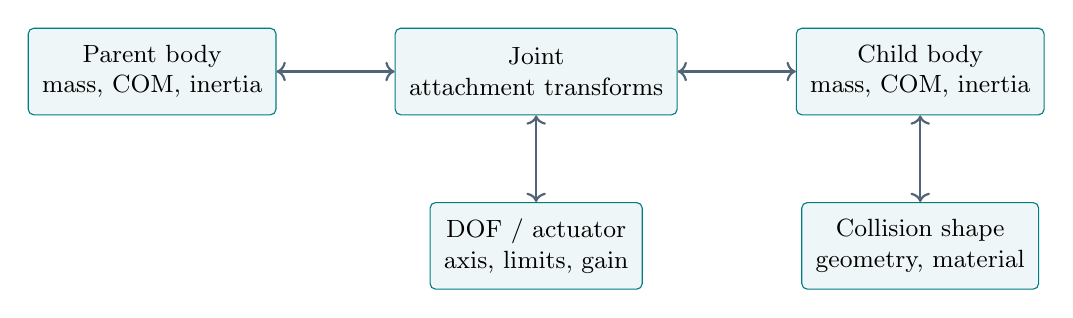
\begin{tikzpicture}[node distance=11mm and 15mm]
\node[box] (parent) {Parent body\\mass, COM, inertia};
\node[box,right=of parent] (joint) {Joint\\attachment transforms};
\node[box,right=of joint] (child) {Child body\\mass, COM, inertia};
\node[box,below=of joint] (dof) {DOF / actuator\\axis, limits, gain};
\node[box,below=of child] (shape) {Collision shape\\geometry, material};
\draw[arr,<->] (parent) -- (joint);
\draw[arr,<->] (joint) -- (child);
\draw[arr,<->] (joint) -- (dof);
\draw[arr,<->] (child) -- (shape);
\end{tikzpicture}
\caption{One illustrative mechanical subgraph. The implementation distinguishes
the two directions of attachment relations. Permitted shape-contact relations
are also represented; they describe eligibility, not the current contact schedule.}
\label{fig:graph}
\end{figure}

Each entity has 104 static slots and 23 dynamic slots, with inapplicable slots
zeroed. A four-way kind indicator identifies the entity type. A separate
24-value global input contains 15 state values and nine context values: counts,
total mass, control/simulation timesteps and gravity. The canonical source
robots have 37 and 46 entity tokens, plus one global token.

\begin{table}[htbp]
\centering\small
\begin{tabularx}{\linewidth}{@{}lYY@{}}
\toprule
Entity & Static examples & Current-state examples\\
\midrule
Body & Mass; COM; full $3\times3$ inertia; dynamic/kinematic flags; root indicator & Root-relative pose; COM linear and body angular velocity; available incoming joint wrench\\
Joint & Type; parent/child attachment transforms; enable flag; DOF dimensions & State is mainly carried by the associated body and DOF tokens\\
DOF & Axis; angular flag; limits; armature; damping; friction; target mode/gains; effort and velocity limits; action gain & Normalized joint coordinate; scaled velocity; previous raw action on actuated DOFs\\
Shape & Primitive; local transform; scale; collision flags; margins; material coefficients; world-shape flag & No independent moving-shape state; attachment connects it to the body\\
\bottomrule
\end{tabularx}
\caption{Information made available to the actor. Availability does not establish
that the trained policy uses each field. Appendix~\ref{app:schema} gives every
static slot and its offset.}
\end{table}

\subsection{Frames, scaling and normalization}
Body positions and orientations are expressed relative to the root link.
Absolute body COM linear velocities and body angular velocities are expressed in
the root axes; these are not velocities with root motion subtracted. Runtime
body quaternions use $wxyz$, while exported Newton transforms use $xyzw$.
The runtime pose encoding chooses a quaternion hemisphere to remove the $q/-q$
ambiguity. These conventions matter when comparing supposedly equivalent models.

Static channels undergo a fixed transform
\begin{equation}
 \widetilde m_{i,r}=\operatorname{sign}(c_r m_{i,r})
                   \log\!\left(1+|c_r m_{i,r}|\right),
 \label{eq:compression}
\end{equation}
with inertia multiplied by 1000 and armature by 100 before compression; other
static channel scales are one. Dynamic channels and the first 15 global values
use empirical normalization. The remaining global context uses signed-log
compression. In the successful imitation experiment, normalization is estimated
from training demonstrations only and then frozen.

These choices make heterogeneous magnitudes easier to process, but they do not
enforce dimensional analysis, unit invariance or a physical computation. A
different unit convention must be mapped to the schema's declared units. Learned
normalization must not absorb validation or target trajectories.

\subsection{Supported scope and caching}
The v1 schema targets rigid articulation trees with supported free, fixed,
revolute and prismatic joints, analytic collision primitives and a flat ground
plane. Mesh geometry, deformables, general closed loops, mimic/tendon mechanisms
and coupled/custom actuation are not represented by this pilot contract. Some
unsupported cases are rejected rather than silently approximated.

The description is cached per prototype. A reset-time or per-world change to
mass, inertia or actuation requires a matching description refresh. Otherwise the
policy receives false information about the simulated system. The relevant
physical attributes belong in the representation; solver caches, rendering data
and arbitrary identifiers do not belong there simply because they are fields on
a Newton model.

\section{Actor architecture and attention}
\label{sec:actor}

\subsection{Exact forward path}
For entity $i$, concatenate compressed mechanics $\widetilde m_i$ and normalized
dynamic state $\widetilde x_i$ and encode them with shared parameters:
\begin{equation}
 h_i^{(0)}=\operatorname{ELU}\!\left(W_e
 [\widetilde m_i;\widetilde x_i]+b_e\right)\in\R^{64}.
 \label{eq:encoder}
\end{equation}
A separate linear projection creates one global token. All tokens then pass
through one local relation-aware attention block and two full-attention blocks.
There are four heads, hence 16 values per head. Each block uses pre-normalization,
a residual attention update, and a residual feed-forward update with width
$64\rightarrow256\rightarrow64$ and GELU activation.

\begin{figure}[htbp]
\centering
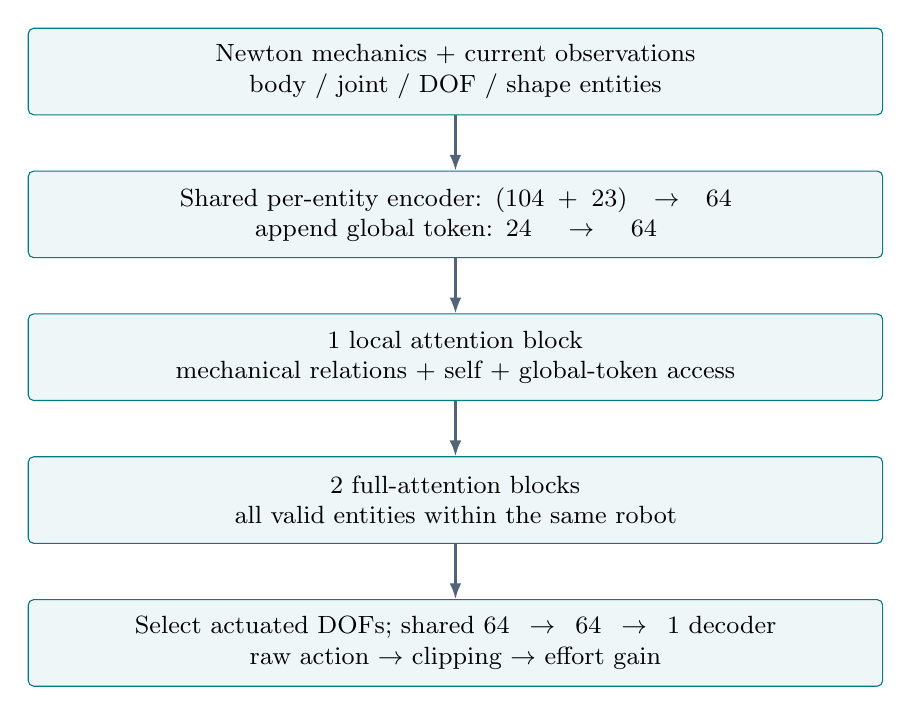
\begin{tikzpicture}[node distance=7mm]
\node[box,text width=105mm] (input) {Newton mechanics + current observations\\body / joint / DOF / shape entities};
\node[box,text width=105mm,below=of input] (embed) {Shared per-entity encoder: $(104+23)\rightarrow64$\\append global token: $24\rightarrow64$};
\node[box,text width=105mm,below=of embed] (local) {1 local attention block\\mechanical relations + self + global-token access};
\node[box,text width=105mm,below=of local] (full) {2 full-attention blocks\\all valid entities within the same robot};
\node[box,text width=105mm,below=of full] (out) {Select actuated DOFs; shared $64\rightarrow64\rightarrow1$ decoder\\raw action $\rightarrow$ clipping $\rightarrow$ effort gain};
\draw[arr] (input) -- (embed);
\draw[arr] (embed) -- (local);
\draw[arr] (local) -- (full);
\draw[arr] (full) -- (out);
\end{tikzpicture}
\caption{The deployed attention actor. Static and dynamic information mix at the
first encoder. There is no temporal memory, predictive world model, or separately
pretrained mechanical encoder in this checkpoint.}
\label{fig:architecture}
\end{figure}

For actuated DOF $k$, the final token is decoded as
\begin{equation}
 a_{t,k}=w_o^\top\operatorname{ELU}
 \left(W_d\operatorname{LN}(h_k^{(3)})+b_d\right)+b_o.
\end{equation}
The same decoder applies to every actuator. Padding is excluded from attention
and masked from actions and PPO action-density calculations. No actor robot ID
or token-position embedding is used. However, counts and geometry can still
identify familiar templates, so absence of explicit IDs does not establish
compositional generalization.

\subsection{What query, key and value mean here}
For one head in a block, let $\bar h_i=\operatorname{LN}(h_i)$ and compute
\begin{align}
 q_i&=W_Q\bar h_i,& k_j&=W_K\bar h_j,& v_j&=W_V\bar h_j,\\
 e_{ij}&=\frac{q_i^\top k_j}{\sqrt{16}}+b_{r(i,j)}+A_{ij},&
 \alpha_{ij}&=\frac{\exp(e_{ij})}{\sum_{\ell}\exp(e_{i\ell})},&
 c_i&=\sum_j\alpha_{ij}v_j.
 \label{eq:attention}
\end{align}
Here $b_{r(i,j)}$ is a learned head-specific relation bias and $A_{ij}$ is zero for
allowed senders and $-\infty$ otherwise. The local block allows mechanical
neighbors, self and global-token connections. The next two blocks allow all valid
tokens in that robot and retain relation biases.

The query specifies what a receiver currently seeks; the key supplies features
against which that request is scored; the value contains the information that
will be communicated. All three derive from mixed mechanics and state, so the
routing can depend on motion as well as structure. Physical connectivity is
known, but task-relevant information flow need not remain local or constant.

For example, a leg actuator could read distant body motion when correcting a
whole-body disturbance. This is a capability of the network, not a measured
interpretation of the learned heads. An attention map alone does not demonstrate
causal physical reasoning. Attention also does not supply a mass matrix, solve
contact constraints, or guarantee extrapolation to a longer kinematic chain.

\subsection{Attention-free and pooling comparisons}
The graph alternative replaces all three attention blocks. Its grouped local
message has the schematic form
\begin{equation}
 c_i^{(g)}=\frac{1}{|\mathcal N_i|}
   \sum_{j\in\mathcal N_i}w_{r(i,j)}^{(g)}
             \phi(\bar h_j)^{(g)},
 \qquad
 \bar h_{\mathrm{global}}=\frac{1}{N}\sum_{j\text{ valid}}\bar h_j.
 \label{eq:message}
\end{equation}
A learned projection of the global mean supplements local messages. The four
groups have 16 channels each, and the message MLP is
$64\rightarrow64\rightarrow64$. Edge-type coefficients are learned but do not
depend on a current receiver/sender query-key comparison. There are no dot-product
attention calls or softmax routing weights in this path.

\begin{table}[htbp]
\centering\small
\begin{tabularx}{\linewidth}{@{}lYYr@{}}
\toprule
Variant & First block & Next two blocks & Parameters\\
\midrule
Attention & Local relation attention & Full relation-biased attention & 164,218\\
Graph & Typed messages + global mean & Same message operation & 164,218\\
Hybrid pooling & Local relation attention & Learned scalar pooling/broadcast & 147,628\\
\bottomrule
\end{tabularx}
\caption{Current actor families. Counts include the shared scalar PPO exploration
parameter. Matching parameter counts does not match FLOPs or isolate a single
operator. The graph implementation uses dense tensors.}
\end{table}

The hybrid pooling actor is not attention-free because its first block is still
local attention. Nor is it a faithful URMA implementation. Both graph and
attention retain individual actuator tokens; neither should be confused with the
older joint-only graph and its 32-value pooled latent.

\subsection{Relation to URMA's routing mechanism}
URMA separately encodes joint descriptions and joint observations. Its encoder
uses descriptor-derived softmax weights to route observation features into a
shared latent; a core network and descriptor-conditioned per-joint decoding then
produce actions~\cite{urma}. This is not the standard pairwise token-to-token
$QK^\top$ operation used in Equation~\eqref{eq:attention}. A useful intuition is
that descriptions identify where a signal should be routed, while observations
supply its changing content. Calling the description a ``key'' is only an
analogy; it should not imply a missing conventional query projection in that
encoder. Our policy instead retains all mechanical entities and lets mixed-state
queries and keys choose their communication. Both designs accommodate variable
input/output counts, but neither property guarantees successful control of any
robot.

\subsection{Training components versus deployment components}
The PPO implementation uses separate flat MLP critics for the prototypes; only
these critics receive prototype indices. A scalar log standard deviation supplies
shared Gaussian exploration for the actor. The critics are not used at
deployment. During imitation, frozen teacher means provide labels, no PPO critic
is trained, and the actor's exploration parameter is unused. The deployed
distilled checkpoint contains one shared actor, not a robot-specific teacher
ensemble or a target adapter.

\section{Specialist-imitation experiment}
\label{sec:protocol}

\subsection{Question and controlled changes}
The diagnostic asks whether the mechanical actors can represent the competent
behavior already found by matched MLP specialists. Student weights start fresh;
the students receive no copied teacher weights. Physical inputs, action mapping,
task and actor architecture are preserved. The change is the learning procedure:
fit teacher action means on collected source states, then execute the fitted
student in the simulator.

The teachers are separate canonical MLP means with widths $[256,128,64]$ from the
common PPO experiment. Their original optimization/exploration machinery was
shared, so they should not be described as fully independent PPO learners. The
fresh evaluations in this study establish the appropriate current reference.

\begin{figure}[htbp]
\centering
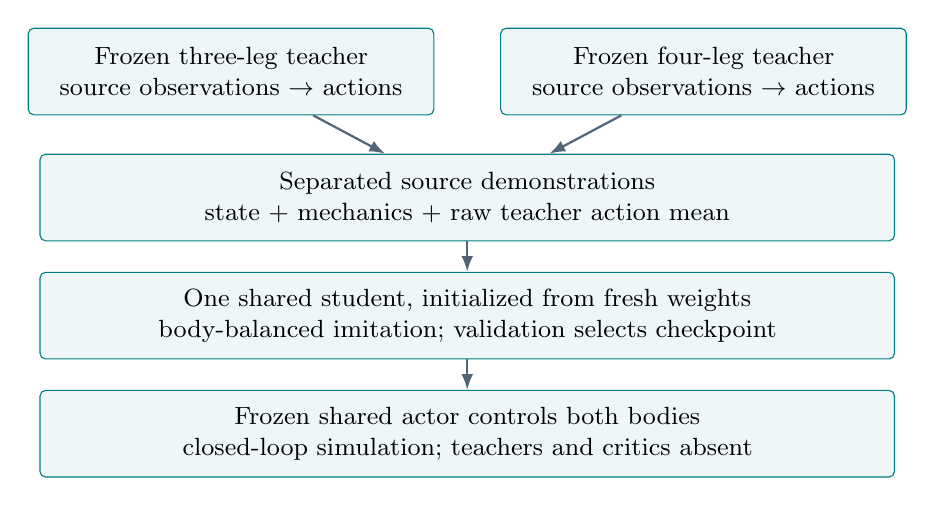
\begin{tikzpicture}
\node[box,text width=48mm] (t3) at (-3,0) {Frozen three-leg teacher\\source observations $\rightarrow$ actions};
\node[box,text width=48mm] (t4) at (3,0) {Frozen four-leg teacher\\source observations $\rightarrow$ actions};
\node[box,text width=105mm] (data) at (0,-1.6) {Separated source demonstrations\\state + mechanics + raw teacher action mean};
\node[box,text width=105mm] (student) at (0,-3.1) {One shared student, initialized from fresh weights\\body-balanced imitation; validation selects checkpoint};
\node[box,text width=105mm] (eval) at (0,-4.6) {Frozen shared actor controls both bodies\\closed-loop simulation; teachers and critics absent};
\draw[arr] (t3) -- (data);
\draw[arr] (t4) -- (data);
\draw[arr] (data) -- (student);
\draw[arr] (student) -- (eval);
\end{tikzpicture}
\caption{Training and deployment are distinct. Teacher action labels guide
supervised fitting; teacher weights are not copied into the student and teachers
are not selected at runtime. This experiment changes learning, not actor size.}
\label{fig:distillation}
\end{figure}

\subsection{Data collection and separation}
For each of four collection reset seeds, run 64 worlds per body for 1,200 control
steps and store every fourth pre-action state. Save raw deterministic teacher
means, executed clipped/scaled efforts, physical descriptors and world/episode
identities. The splits are:
\begin{table}[htbp]
\centering
\begin{tabular}{@{}lrrl@{}}
\toprule
Split & Reset seeds & States per body & Use\\
\midrule
Training & 1011, 2022 & 38,400 & Gradients and normalization\\
Validation & 3033 & 19,200 & Checkpoint selection\\
Source-state test & 4044 & 19,200 & Action-error reporting\\
\bottomrule
\end{tabular}
\caption{Entire collection runs are separated. A source-state test is not an
unseen-morphology test. No five-leg data enter this study.}
\end{table}

The four collections consume 614,400 simulator transitions in total, including
validation/test collection. The teachers previously used 16.384 million training
transitions. Repeated presentations of stored examples add optimizer work, not
new environment transitions.

\subsection{Body-balanced loss and fitting}
For a batch of $B$ bodies with $n_b$ examples and $K_b$ valid actuators, the loss is
\begin{equation}
 \mathcal L_{\mathrm{BC}}=
 \frac{1}{B}\sum_{b=1}^{B}\frac{1}{n_b}\sum_{t=1}^{n_b}
 \frac{1}{K_b}\sum_{k=1}^{K_b}
 \left(\policy(o_{b,t},\mech_b)_k-a^*_{b,t,k}\right)^2.
 \label{eq:bc}
\end{equation}
Thus, a longer action vector does not automatically dominate training. Targets
are raw teacher means, not clipped efforts: previous raw action is observed and
raw action penalties also affect the task.

Each main fit runs 6,000 Adam steps with 128 sampled examples per body per step,
or 768,000 sample presentations per body with replacement. The learning rate
decays by cosine from $3\times10^{-4}$ to $3\times10^{-5}$; gradient norm is
limited to one. Normalizers are computed once from training data and frozen.
Checkpoints are selected by minimum mean validation action MSE at step 1 and
every 250 steps. All five main fits selected step 6,000.

The conditions are a shared attention student, a shared graph student, a separate
graph for each body, and a separate-MLP-means imitation control. Each separate
graph owns a full network; their combined parameter count is twice that of one
shared graph. Separate versus joint fitting also changes normalization, so the
comparison does not isolate gradient interference alone.

\subsection{Rollout and implementation checks}
Selected checkpoints are frozen and evaluated for 1,200 steps with 64 worlds per
body and reset seeds 123, 456 and 789. These evaluation trajectories do not select
checkpoints. The queue completed 28 jobs: four collections, six fits including a
small memorization check, and 18 teacher/student evaluations.

The recorded checks cover body-balanced loss, padding gradients, raw-versus-clipped
targets, collection-split rejection, checkpoint restoration and frozen
normalization. Stored states reproduce teacher labels within $7.8\times10^{-7}$
across the checked CPU/GPU paths. Descriptor comparison tolerates absolute
$10^{-12}$ transform roundoff with zero relative tolerance; integer topology is
exact. This addressed a $1.4\times10^{-17}$ translation discrepancy without
permitting a changed robot. A 64-state-per-body memorization check reached
training RMSE 0.036/0.047 after 1,000 updates. It is a fitting check, not a new
locomotion candidate.

\section{Results and what they establish}
\label{sec:results}

\subsection{Source control after distillation}
\begin{table}[htbp]
\centering\small
\begin{tabular}{@{}lrrrr@{}}
\toprule
 & \multicolumn{2}{c}{Three legs} & \multicolumn{2}{c}{Four legs}\\
\cmidrule(lr){2-3}\cmidrule(l){4-5}
Controller & m/s & Survival (\%) & m/s & Survival (\%)\\
\midrule
\tableinput{generated/source_results.tex}
\bottomrule
\end{tabular}
\caption{Fresh frozen-checkpoint evaluations from the October 7 diagnostic.
Values are means over three evaluation reset runs. The table is generated from
the included result snapshot rather than copied manually.}
\label{tab:source}
\end{table}

The attention student satisfies the numerical source criteria on both canonical
bodies. The shared graph recovers 97.2\% and 95.4\% of teacher speed, but its
three-leg survival is below 95\%, and both bodies lose more than two percentage
points against their teachers. Attention is therefore the current engineering
baseline; the result does not establish universal architectural superiority.

\begin{figure}[htbp]
\centering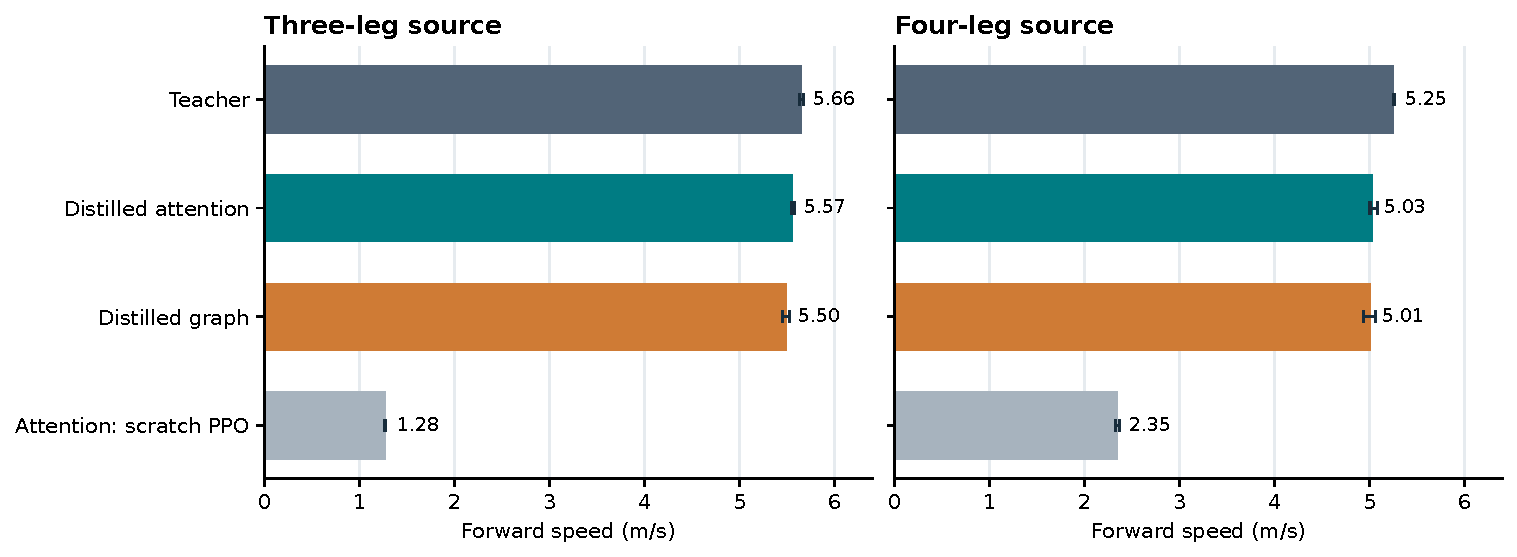
\includegraphics[width=\linewidth]{figures/source_speed.pdf}
\caption{Source speed under the teacher, two distilled actors, and the earlier
scratch-PPO attention policy. Whiskers show the minimum/maximum reset-run means,
not confidence intervals over retraining. Distillation includes teacher and data
collection costs, so this is a learning-procedure diagnostic, not an equal-cost
algorithm ranking.}
\label{fig:speed}
\end{figure}

\begin{figure}[htbp]
\centering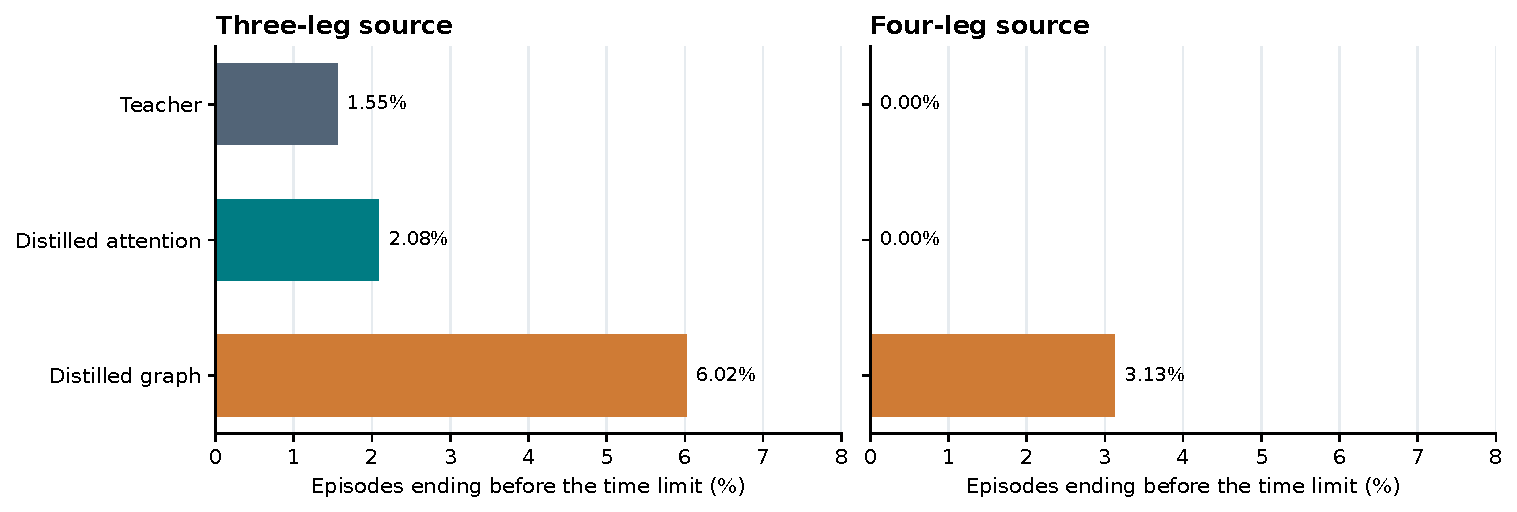
\includegraphics[width=\linewidth]{figures/source_failure.pdf}
\caption{The complement of reported time-limit survival. Graph imitation retains
fast motion but has more early-ending episodes. Zero observed early endings is
not a guarantee of failure-free operation.}
\label{fig:failure}
\end{figure}

\FloatBarrier
\subsection{Action-fitting error}
\begin{table}[htbp]
\centering\small
\begin{tabular}{@{}lrrrr@{}}
\toprule
 & \multicolumn{2}{c}{Three legs} & \multicolumn{2}{c}{Four legs}\\
\cmidrule(lr){2-3}\cmidrule(l){4-5}
Student & Raw RMSE & Relative (\%) & Raw RMSE & Relative (\%)\\
\midrule
\tableinput{generated/imitation_errors.tex}
\bottomrule
\end{tabular}
\caption{Held-out source-state action errors. Relative RMSE divides by the
training-label standard deviation; it is not a control success rate.}
\end{table}

The shared attention student fits the actions better than the shared graph, while
both remain less accurate than the MLP control. Closed-loop outcomes are still
necessary: errors on teacher-visited states do not capture state-distribution
drift or recovery after an unusual student action. Small action MSE does not
guarantee stability.

\subsection{Earlier PPO architecture and diversity screen}
\begin{table}[htbp]
\centering\small
\begin{tabular}{@{}rlrrr@{}}
\toprule
Sources & Actor & Three legs & Four legs & Five-leg development\\
\midrule
\tableinput{generated/ppo_results.tex}
\bottomrule
\end{tabular}
\caption{Earlier mechanical-policy PPO runs: speed in m/s / survival in percent.
Each uses 500 updates, 16.384 million aggregate transitions and training seed 42.
These five-leg results do not describe the later distilled checkpoints.}
\label{tab:ppo}
\end{table}

The graph improves some source measurements under PPO but has no consistent
transfer advantage. Its five-leg speed falls sharply in the eight-prototype run
despite 100\% survival. Because aggregate experience is fixed, eight prototypes
receive one quarter the per-prototype exposure of the two-prototype run. More
diversity and less per-body experience change together, so this is not an
isolated causal test of diversity.

An earlier joint-only graph was also extended from 500 to 2,500 updates. Solo
three-/four-leg speeds rose from 1.502/2.544 to 1.880/3.895\,m/s; shared speeds
rose from 1.732/2.149 to 2.308/3.310\,m/s. Longer training helped that architecture,
with smaller late gains, but it remained a different representation from the
current mechanical actor. Those results neither establish nor rule out the value
of longer training for the new learning recipe.

\subsection{Earlier inertial-feature ablation}
For eight-source attention/PPO, removing mass, COM, inertia, armature and total
mass inputs changed canonical three-/four-leg and development five-leg speeds
from 1.089/2.996/0.875 to 1.895/2.094/0.170\,m/s. Three legs improved while four
and five legs worsened. This is mixed evidence for the utility of those inputs,
not proof of a learned inertial model. The ablation retrains PPO, changes learning
dynamics, and still supplies geometry and dynamic state that can reveal physical
properties. It has not been repeated on the successful distilled baseline.

\subsection{Interpretation limits}
The positive source result refutes a categorical claim that the current shared
architecture cannot express the fast source behaviors. It does not distinguish
exploration, credit assignment, normalization, optimizer behavior and cross-body
interference: imitation changes several of these together. Nor does it show that
an unseen body is controlled using its mechanics rather than template recognition.
Older specialists at roughly 6.25/5.37\,m/s used a different contract; the freshly
evaluated teachers in Table~\ref{tab:source} are the appropriate local reference.

\section{Frozen transfer to additional robots: October 7 extension}
\label{sec:transfer}

The same source-selected attention and graph checkpoints were applied to the
five-leg development Ant and to Unitree Go2 and A1 USD assets. No target data
entered fitting, normalization or checkpoint selection. The actor, normalizers
and output decoder were unchanged; the graph supplies ten actions for five-leg
Ant and twelve for both Unitree models. This extends the accepted interface,
but does not establish successful behavior on those robots.

\paragraph{Physical and evaluation contract.}
Each target/controller uses reset seeds 123/456/789, 64 worlds per run and
1,200 control steps at 60 Hz, with a 16-second episode limit and early resets.
These are reset repetitions, not new training seeds. Speeds in
Table~\ref{tab:transfer} divide completed-episode progress by completed-episode
time, then average the three run-level ratios. Survival is the fraction of
completed episodes reaching the time limit. Mean episode duration is essential
for interpreting a policy that repeatedly falls; negative speeds during those
falls are not a backward locomotion gait. The data snapshot also contains
progress over the entire rollout, including unfinished episodes, and action
saturation rates.

\begin{table}[htbp]
\centering\small
\begin{tabular}{@{}llrrr@{}}
\toprule
Target & Actor & Speed (m/s) & Survival (\%) & Episode (s)\\
\midrule
\tableinput{generated/transfer_results.tex}
\bottomrule
\end{tabular}
\caption{Frozen distilled actors on development targets. Unitree rows use the
explicit simulated effort-control conversion below, not stock hardware drives.}
\label{tab:transfer}
\end{table}

Unitree geometry, masses, joint layout, nominal posture and configured effort
limits are retained. Their stock DC motor/position controllers are replaced by
ideal effort control with 0.1 N\,m\,s/rad damping, matching the Ant's damping
convention. This is a declared model conversion, not an exact stock-motor test.
The existing descriptor has four drive-mode slots and rejects Newton's fifth,
pure-effort mode; it can encode the velocity-drive mode used for this damping.
No field was silently remapped or added to the trained network.

Unitree simulation uses 480 Hz integration while preserving 60 Hz policy
updates. The original 120 Hz integration produced non-finite Go2 observations
under large efforts. Constraint/contact capacities were increased to
2,048/256 per world after a capacity overflow in an initial probe. Failed probes
are retained in the logs and excluded from scores. Ant integration remains
120 Hz. Both the physics settings and descriptor values are recorded per run.

The standing sanity check uses nominal-posture PD effort feedback at every
Unitree physics step, with gains 25 and 0.5. It is an environment check, not a
trained locomotion specialist or an equal-controller comparison. Go2 reaches
100\% survival with this controller. A1 reaches only 16.6\% with the same gains;
a separate follow-up raising only its standing feedback damping to 2.0 reaches
100\% survival over 64 worlds at reset 123. The learned-policy plant and weights
are unchanged. This follow-up was prompted by the failed standing check and is
not part of the original three-reset matrix. Neither target had a matched
trained locomotion specialist in this frozen experiment; the later Go2
reference is established in Section~\ref{sec:go2learning}.

\begin{finding}{Interpretation}
Source imitation solves the earlier source-performance gap but does not solve
transfer. The five-leg robot largely remains above its fall-height threshold
while moving slowly. Both shared actors fall rapidly on the new quadruped
family. The result does not isolate training coverage, mechanical reasoning,
coordinate conventions, rich-state normalization or effort-control semantics
as the cause. It motivates a controlled new-family learning comparison before
another increase in network size.
\end{finding}

The targets are now development data. The reserved five-leg parameter
combinations remain untouched. The new evaluation tool is
\path{scripts/tools/evaluate_mechanical_transfer.py}; raw reports, failed setup
probes, descriptor tensors, fixed-world videos and a gallery are under
\path{logs/shared_ant_graph/other_robots_20261007/}. The portable report includes
\path{data/transfer_summary.json}, with the frozen protocol and compact reports.

\section{Learning a new family: Go2 specialist and distillation}
\label{sec:go2learning}

This extension separates learning the new robot from sharing its controller with
the Ant family. Go2 becomes a training body. A1 and five-leg Ant remain
development transfer probes, with no demonstrations or normalization samples used
for either fit. Previously inspected development bodies are not an untouched
confirmation suite.

\subsection{A competent reference under the declared task}
A conventional Go2 MLP specialist uses the same rich observations, ideal effort
mapping, reset distribution, reward and 480\,Hz physics/60\,Hz control as the
frozen transfer study. The actor has layers 256--128--64 and 124,621 parameters.
It uses 1,024 worlds, 32-step PPO rollouts and seed 42. The first 500 updates
(16.384 million transitions) produce stable standing but essentially zero
forward speed. This fails the predeclared collection gate: mean speed at least
1\,m/s and mean time-limit survival at least 95\%.

A documented continuation adds 1,000 updates with the same weights, optimizer,
normalizers and training configuration, restarting the simulator rollout state.
At 1,500 total updates (49.152 million transitions), the frozen final checkpoint
reaches 9.921\,m/s and 100\% survival across reset seeds 123/456/789.
This establishes learnability of the simulated task. It is not a prediction of
real Go2 performance: the converted model omits the stock motor torque--speed
curve, and the objective maximizes forward progress rather than tracking a
bounded speed command. Longer training helped this specialist; the result does
not establish that duration alone repairs the shared student's learning problem.

\subsection{Controlled imitation comparison}
The two students are fresh copies of the existing 164,218-parameter attention
actor, each initialized with seed 42. One fits Go2 only; the other fits Ant3,
Ant4 and Go2. Architecture, token schema, action decoder and training objective
are unchanged. Four Go2 collections use 64 worlds, 1,200 control steps and
sampling every fourth step: 307,200 new simulator transitions in total. Seeds
1011/2022 supply training data, 3033 validation and 4044 test data. Each body has
38,400 training rows and 19,200 rows per held-out split. Existing Ant collections
are reused without changing their 120\,Hz physics. Both families retain 60\,Hz
actions.

Stored graph layouts reproduce the live mechanical encoder exactly on checked
observations. Descriptor snapshots, teacher hashes, dependency versions and
observation widths are verified before fitting. This permits offline mixed-body
batches without forcing Ant and Go2 to share a simulator integration timestep.

Each fit uses 6,000 Adam updates, 128 samples per body per update, a learning rate
decaying from $3\times10^{-4}$ to $3\times10^{-5}$, and equal body weighting of
valid-DOF raw action MSE. The selected checkpoint minimizes source validation
MSE, not rollout performance. Normalization is estimated only from that
condition's training demonstrations and then frozen. Both conditions therefore
have 768,000 Go2 sample presentations, but the joint condition has three times
as many total presentations and different normalization statistics. It is a
useful system comparison, not an isolated gradient-interference ablation or an
equal-total-compute comparison.

\subsection{Frozen rollout results}
\begin{table}[htbp]
\centering\small
\begin{tabular}{@{}lrrr@{}}
\toprule
Robot & Specialist & Go2-only attention & Shared Ant+Go2\\
\midrule
\tableinput{generated/go2_learning_results.tex}
\bottomrule
\end{tabular}
\caption{Speed (m/s) / 16-second survival (\%). Each cell averages three
reset runs, 64 worlds per body and 1,200 steps. Dashes denote unmeasured cells or
missing matched references. Ant evaluation preserves the canonical paired-source
layout; the Go2 teacher is the longer-trained reference above. These are fixed
trained policies, not independent training replicates.}
\label{tab:go2learning}
\end{table}

The Go2-only student has a held-out raw-action RMSE of approximately 0.018,
yet fails to sustain locomotion. Small average error on expert trajectories is
insufficient to establish closed-loop control. Because this failure occurs
without Ant sharing, interference between embodiments cannot be its sole cause.
Neither architecture capacity nor the proposed mechanical representation has
been isolated as the cause by this comparison.

The mixed fit retains Ant speeds of 5.467/5.086\,m/s, but Ant3/Ant4 survival falls
to 89.81\%/96.35\%, versus 97.9\%/100\% for the earlier Ant-only attention
checkpoint. Both fail the full source acceptance rule: Ant3 misses 95\%
survival, and Ant4 loses more than two percentage points relative to its teacher.
Joint training was fresh, with Ant replay throughout; this is not a sequential
fine-tuning/forgetting experiment. Go2-only and shared Go2 episodes last only
0.680 and 0.212 seconds, respectively. A1 still falls rapidly and five-leg
progress remains 0.131\,m/s. The new shared checkpoint therefore does not replace
the Ant-only incumbent.

\paragraph{Fresh trajectory diagnostic.}
A post-matrix check uses reset 123, 64 worlds and 1,200 steps per condition,
executing either the teacher or student while evaluating both actors' actions.
All weights and normalizers remain frozen. For Go2-only imitation, RMSE is
0.01950 on teacher-visited states and 0.27446 on student-visited states. The
shared actor gives 0.04397 and 0.24865, respectively. On teacher trajectories,
Go2-only error in the first 0.25 seconds is 0.04778, versus about 0.017 after
one second. This supports examining startup coverage and state-distribution
drift; it does not isolate a unique cause. Different behavior policies visit
different states, and expert actions on fallen student states are not guaranteed
optimal recovery labels. These four diagnostic rollouts add 307,200 simulator
transitions, with no fitting or checkpoint selection. See
\path{data/go2_diagnostics.json}.

\begin{figure}[htbp]
\centering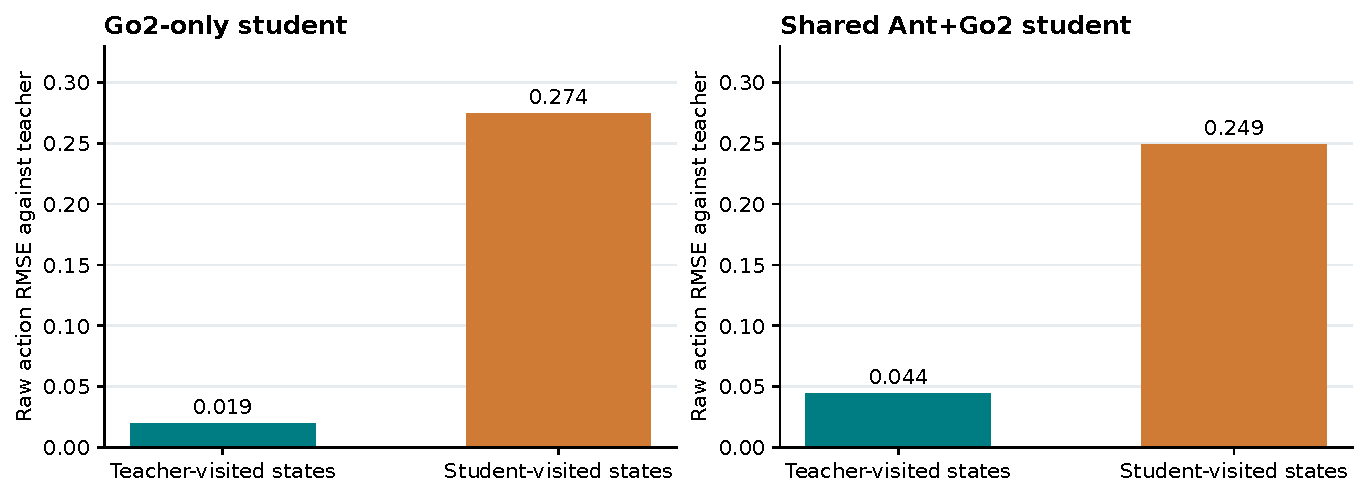
\includegraphics[width=\linewidth]{figures/go2_rollout_error.pdf}
\caption{The small action errors on fresh expert trajectories do not persist
on trajectories controlled by the students. RMSE is in dimensionless raw-action
units. These are post-matrix diagnostics for the fixed checkpoints, not causal
proof that dataset coverage alone explains the failures.}
\label{fig:go2error}
\end{figure}

The next learning intervention should explicitly cover startup and
student-visited recovery states, retaining Ant replay. Compare fitting augmented
demonstrations with an equal-update continuation on the original data to
distinguish additional state coverage from simply adding optimizer steps.
Teacher actions on arbitrary fallen states are not guaranteed recovery targets;
report expert recoverability and any assisted-rollout schedule. Preserve the
current checkpoints, keep A1 out of fitting, and select checkpoints using source
validation. This is a proposed repair of imitation learning, not a new-algorithm
claim or evidence of universal transfer.

The complete protocol, checkpoints, raw reports and fixed-world videos are under
\path{logs/shared_ant_graph/go2_learning_20261007/}. Tools are
\path{scripts/tools/train_mechanical_go2.py} and
\path{scripts/tools/distill_mechanical_cross_family.py}; the portable result
snapshot is \path{data/go2_learning_summary.json}.

\FloatBarrier
\section{Capabilities, limitations and failure modes}
\label{sec:gaps}

\begin{longtable}{@{}p{0.29\linewidth}p{0.66\linewidth}@{}}
\toprule
Question & Current evidence or gap\\
\midrule
\endhead
One policy, several action counts & Demonstrated source control on six- and
eight-action Ants; the interface accepts ten-action Ant and twelve-action Unitree variants.\\
Unseen morphology & Frozen distilled actors crawl on five legs and fail on the
simulated Unitree targets; see Section~\ref{sec:transfer}.\\
Mechanical conditioning & Rich fields are exported. Their compositional use by
the successful actor is unproven.\\
Embodiment diversity & Eight earlier prototypes still mean two source topologies;
the successful distilled actor sees only the canonical pair. Adding Go2 has been
tested, but the mixed fit is not competent on all three sources.\\
Physical-description consistency & Token permutations and padding are tested.
Arbitrary body frames, axis signs and fixed-link decomposition have no guarantee.\\
Sensing and hidden dynamics & Current state is simulator-rich. No history or
online system identification addresses uncertain mechanics or missing sensors.\\
Model coverage & General constraints, coupled actuators, deformables and mesh
geometry require new schema/control support.\\
Practical compute & Actor parameter counts are known. Batch-one latency, control
deadline headroom and broad scaling are not characterized.\\
Task coverage & Forward progress only. Command following, terrain, manipulation
and hardware deployment have separate requirements.\\
Transfer efficiency & Earlier target-adapter pilots motivate reuse; the distilled
mechanical actor has not established target-sample savings or a frozen-core benefit.\\
\bottomrule
\end{longtable}

The strongest risks are not merely model size. Template shortcuts can make a
mechanics-rich network appear physically informed. Cached descriptions can become
stale under randomization. Coordinate-dependent numbers can make equivalent
robots look different. Teacher-state coverage can leave the student unprepared
for recovery. An implementation that accepts a graph does not resolve any of
these issues automatically.

Attention is a useful flexible communication mechanism, but there is no current
reason to treat it as mandatory. Conditional parameters, deterministic mechanical
canonicalization, better data coverage or an improved training objective may be
more effective than adding heads or layers. A change should address a measured
failure and retain a matched simple control.

\section{Related work and novelty assessment}
\label{sec:novelty}

\subsection{What the current ingredients already overlap}
Structured graph control is established by NerveNet~\cite{nervenet}.
Morphology-conditioned Transformer control and contextual modulation appear in
MetaMorph and ModuMorph~\cite{metamorph,modumorph}. URMA supplies a particularly
relevant shared locomotion architecture~\cite{urma}. Our explicit body, DOF and
shape representation is a design choice to evaluate; a richer descriptor list
alone is not a demonstrated research contribution.

The closest precedent to the successful learning recipe is
UniLegs~\cite{unilegs}: specialist locomotion policies are distilled into a shared
Transformer. Its proprioceptive, joint-target setting differs from our richer
body/wrench observations and effort actions. These differences prevent a direct
performance ranking and require task-matched tests. Its normalized-reward results
cannot be compared numerically with our teacher-normalized speeds. Our present
finding validates this implementation's source capability; it does not introduce
specialist-to-Transformer distillation.

\begin{table}[htbp]
\centering\small
\begin{tabularx}{\linewidth}{@{}p{0.29\linewidth}YY@{}}
\toprule
Reference family & Relevant overlap & Implication\\
\midrule
NerveNet; MetaMorph; ModuMorph & Graph sharing, morphology conditioning and
attention & These are baselines, not stand-alone novelty claims.\\
URMA & Shared locomotion with variable input/output counts & Variable-size control
requires an empirical advantage beyond interface generality.\\
UniLegs & Specialist-to-shared-policy distillation & Our successful recipe has a
close prior precedent.\\
Embedding Morphology into Transformers~\cite{embedding} & Joint tokens,
topology-biased attention and attribute conditioning & Combining graph relations
and descriptors with attention is also established.\\
Graph physics; QWM~\cite{graphphysics,qwm} & Learned physical dynamics and
morphology-conditioned world models & Adding a predictor is not sufficient.\\
CMIRL; GraphOp-WM~\cite{cmirl,graphop} & Mechanical interventions, structured
morphology pathways and paired-morphology supervision & Counterfactual mechanics
training needs a narrower distinction.\\
MS-PPO~\cite{symmetry} & Graph policies respecting morphological symmetry &
Equivariance alone is not a new contribution.\\
\bottomrule
\end{tabularx}
\caption{Targeted primary-source comparison as of the report date. We have not
reproduced these methods under a common benchmark.}
\end{table}

\subsection{Why a generic physics auxiliary objective is insufficient novelty}
Graph networks have long been used for physical inference and
control~\cite{graphphysics}. QWM conditions a quadrupedal world model on morphology
and uses the learned dynamics for policy learning~\cite{qwm}. CMIRL separates
morphology and shared-mechanism pathways and uses simulator morphology
interventions~\cite{cmirl}. GraphOp-WM combines attributed body graphs, structured
operators and paired-morphology supervision, with controlled parameter-composition
splits~\cite{graphop}. Consequently, neither ``mechanics plus a world model'' nor
``learn from counterfactual physical changes'' is a defensible broad novelty
claim for our next experiment.

A more specific possibility is that \emph{local mechanical effects learned on
source structures transfer to different articulated topologies}, while physical
control remains insensitive to arbitrary description conventions. That claim
would require a defined mechanism, structural tests and matched alternatives;
it is not established by our current source results.

\subsection{Different types of possible contribution}
An algorithmic contribution needs a new mechanism with a controlled benefit over
stronger existing alternatives. An empirical contribution could identify when
mechanical context helps, when it is redundant with state, or when optimization
prevents its use. A benchmark/schema contribution could expose failures caused by
equivalent model descriptions and supply validated transformation pairs. The
current Newton exporter and experiment tooling are enabling infrastructure, not
evidence that any of those contributions has already been achieved.

The literature check is targeted rather than exhaustive. In particular,
description-frame consistency must be distinguished from morphological symmetry:
the former can arise for an asymmetric robot because coordinate frames are a
modeling choice. Existing symmetry-aware locomotion methods remain important
comparators~\cite{symmetry}. No first-of-kind claim is made for the proposed
combination.

\section{Proposed research directions}
\label{sec:proposals}

\begin{finding}{Proposed work: not implemented or evaluated}
The two directions below are hypotheses to test using the source-competent actor.
The existing checkpoint has no predictive auxiliary head or enforced local-frame
equivariance. A successful source gait is a starting point, not evidence for
either proposed property.
\end{finding}

\subsection{A: local mechanical interventions and structural transfer}
\label{sec:interventions}
The first hypothesis is that learning the effect of a local physical change can
encourage a representation that transfers beyond recognizing source templates.
Begin with fixed topology and geometry while changing valid payload/inertia and
actuator parameters. Hold out parameter combinations. If the existing
direct-conditioned actor already handles them, retain that simpler method.

For a matched simulator state $s$ and physical control $u$, a pure inertial
intervention gives
\begin{equation}
 \Delta y=y\!\left(F_{\mech'}(s,u)\right)
          -y\!\left(F_{\mech}(s,u)\right),
 \label{eq:paired}
\end{equation}
where $y$ extracts corresponding body/joint velocity features in consistent
coordinates. Each pair has the same topology, so its correspondence is explicit.
Train on many such local pairs from source structures, then test whether the
learned relation transfers to a new structure. Do not define a naive elementwise
subtraction between states with different numbers of joints.

For motor-strength changes, holding normalized action $a$ fixed intentionally
changes $u=C_{\mech}(a)$ through the execution mapping. That is a different paired
experiment and must be labeled accordingly. For inertial changes, hold applied
effort fixed. Density interventions must update mass and inertia together;
payload changes must produce a physically realizable COM and inertia. Contact
state, constraint caches and derived wrench observations must be handled
consistently when cloning and modifying a simulator state.

A possible auxiliary objective is
\begin{equation}
 \mathcal L_{\mathrm{paired}}=
 \left\|D_\theta(s,u,\mech')-D_\theta(s,u,\mech)-\Delta y\right\|_W^2,
 \qquad
 \mathcal L=\mathcal L_{\mathrm{BC}}+\lambda\mathcal L_{\mathrm{paired}}.
 \label{eq:pairedloss}
\end{equation}
$W$ declares feature scales rather than allowing the largest physical units to
dominate. This is a candidate implementation, not a completed method. Compare it
with ordinary next-state prediction using the same transitions and a matched
prediction head. Dynamics prediction can improve without improving control, so
held-out closed-loop performance is the decisive measurement.

\textbf{Controls.} Use direct-conditioned imitation, ordinary prediction plus
imitation, and paired prediction plus imitation. Match teacher access, actor/head
capacity, source data and simulator queries; count both branches of each paired
simulation. Teacher labels must be generated by competent policies for the
actual physical variants. Canonical teacher actions are not automatically expert
labels for a heavier or weaker robot. Strict zero-shot tests allow no target
dynamics queries in source training or checkpoint selection.

\textbf{Success and falsification.} Success is better control/survival on locked
parameter combinations and new structures, with correct mechanical context
materially useful. If only prediction improves, if matched-data controls erase
the gain, or if removing inertial/actuator information preserves the result,
the proposed mechanism has not earned its claimed role. Structural reuse, rather
than counterfactual supervision by itself, is the proposed distinction from the
nearby work discussed in Section~\ref{sec:novelty}.

\subsection{B: equivalent-description consistency}
\label{sec:equivalence}
The second hypothesis is that mechanically equivalent descriptions should lead
to equivalent physical control. Let $T$ change model coordinates without changing
the robot, and let $T_a$ map actions consistently. The desired property is
\begin{equation}
 \policy(T_s s,T_\mech\mech)\approx T_a\policy(s,\mech).
 \label{eq:equivariance}
\end{equation}
When $T_a$ is nontrivial this is equivariance, not literal equality of action
numbers. Our tested token-permutation property is only one special case.

For a scalar joint-axis reversal, an illustrative consistent mapping is
\begin{equation}
 q'=-q,\quad \dot q'=-\dot q,\quad
 [q'_{\min},q'_{\max}]=[-q_{\max},-q_{\min}],\quad u'=-u.
\end{equation}
The joint axis, reference configuration, previous action and other directional
quantities must also transform consistently. For a local body-frame rotation,
poses, attachment transforms, axes, COM vectors, inertia tensors and wrench
components require corresponding transformations. Transforming only a few input
vectors would describe a different physical system.

First verify generated pairs through forward kinematics and short dynamics
checks under mapped actions. Then measure action disagreement after mapping both
outputs to a common physical convention, followed by rollout speed and survival.
This separates an incorrect transformation generator from a policy inconsistency.

\textbf{Candidate remedies.} Compare deterministic canonicalization, consistent
data augmentation, and a learned encoder or consistency penalty enforcing
Equation~\eqref{eq:equivariance}. A canonical frame cannot simply be assumed to be
unique for symmetric or degenerate geometry; the convention and ambiguous cases
must be explicit. A possible training penalty is
\begin{equation}
 \mathcal L_{\mathrm{equiv}}=
 \mathbb E_{s,\mech,T}\!\left[
 \|\policy(T_s s,T_\mech\mech)-T_a\policy(s,\mech)\|^2\right].
\end{equation}
This penalty alone admits unhelpful constant policies, so it must be paired with
competent task/imitation performance and tests of sensitivity to real mechanics.

Fixed-link merging/splitting is a later, harder test. Combined spatial inertia,
collision surfaces and constraints must remain equivalent, and numerical solver
effects can break an assumed equivalence. Duplicating collision shapes is not a
valid shortcut because it can change contacts. Start with exact coordinate
re-expressions rather than ambiguous model edits.

\textbf{Success and falsification.} Success is lower physical-action/rollout
discrepancy on equivalent descriptions, without losing source competence or
useful response to actual physical changes. If ordinary canonicalization solves
the issue, that is the preferred remedy. If the baseline is already sufficiently
consistent, a new network is not justified. A contribution may lie in a validated
schema and benchmark rather than a more complicated actor.

\subsection{Why the two requirements belong together}
A representation should ignore arbitrary conventions while retaining information
that changes dynamics. Insensitivity to everything would pass a superficial
invariance test but be useless for adapting to a heavier link. Sensitivity to
every descriptor perturbation would react to coordinate choices that do not
change the robot. Evaluating both properties, and then structural transfer,
offers a stronger test of reusable mechanics than either input ablation or
attention visualization alone.

\section{Ordered experiment program}
\label{sec:plan}

The following program is conditional. It uses the current trained checkpoints
first and introduces new training only when a measurement identifies a specific
gap. No independent-seed sweep is included.

\subsection{Phase 1: freeze and measure the current actors}
\textbf{Completed in the transfer extension.} Section~\ref{sec:transfer} records
the target measurements; the following paragraph preserves the stage's protocol.
Freeze the distilled attention and graph checkpoints, normalization and selection
rule. Evaluate canonical sources and the existing five-leg development body with
matched resets. Record speed, survival, action saturation and fixed-reset videos.
The canonical evaluations already exist; repeat them only as needed to check a
new evaluation path, rather than spending compute on redundant measurements.

\textbf{Decision:} does successful source imitation transfer at all? A negative
five-leg result motivates representation/coverage work. A positive result is a
development finding, not an untouched structural test or evidence of arbitrary
robot control.

\subsection{Phase 2: audit mechanics and conventions without retraining}
Construct bounded, physically valid fixed-topology variants. For the same actual
simulated variant, compare correct descriptions with deliberately mismatched
descriptions that represent other valid variants. Keep observations and all
non-target fields consistent. Separately apply validated equivalent-coordinate
transformations and map the actions back.

\textbf{Decision:} are physical fields useful, ignored, or associated with brittle
out-of-distribution behavior? Inference-time swaps are sensitivity probes, not
conclusive causal evidence, because the mismatch itself creates distribution
shift. A small action change can be appropriate under a robust policy; require a
control-relevant effect rather than rewarding sensitivity for its own sake.

\subsection{Phase 3: separate physics variation from template identity}
Build a small factorial source population varying payload/inertia and motor
strength while geometry is held fixed. Define held-out combinations before
training. Validate physical realizability and descriptor refresh, then obtain
competent per-variant teacher coverage. Train full-mechanics and geometry-only or
masked-mechanics actors on identical observations, labels and sample counts.

\textbf{Decision:} does explicit mechanics improve control beyond identifying a
template? Rich dynamic observations may still reveal physical properties, so a
negative ablation limits the claim in this sensing/task regime, not in every
possible partially observed setting. If variants lack competent teachers,
resolve that reference failure before attributing poor students to sharing.

\subsection{Phase 4: test one justified mechanism}
Choose direction A when composition fails despite informative mechanical inputs.
Choose direction B when equivalent descriptions cause meaningful discrepancies.
Retain a direct-conditioned or canonicalized control. Change one principal
mechanism at a time and compare data, capacity and compute explicitly.

If student state drift is the main failure, collect teacher labels on
student-visited/recovery states, following the motivation of dataset aggregation
methods such as DAgger~\cite{dagger}. This is a targeted repair, not a novelty
claim. Imitation-initialized PPO is justified by a measured teacher ceiling or
task mismatch; monitor whether early updates destroy the competent gait.

\subsection{Phase 5: test new structures under a locked recipe}
After development choices are fixed, evaluate a broader family-held-out suite:
new leg counts, link counts, branching patterns, and eventually other supported
body families. Separate parameter interpolation, parameter extrapolation,
unseen combinations and structural change. If five-leg robots enter training,
the old five-leg development result becomes within-topology evidence.

Compare against a credible shared morphology-conditioned/distilled baseline
under the same inputs, control semantics, teachers and budgets. A port with
substantial changes should be called a literature-aligned baseline rather than an
exact reproduction. Use target specialists only for isolated scoring; their
trajectories and model-selection signals must not leak into a zero-shot actor.

Report per-body results, minimum/median teacher-normalized speed, survival and
failures. A sufficiently broad suite is needed before a lower-decile statistic
is meaningful. Preserve both fixed-total-budget and fixed-per-body-budget
comparisons when growing populations; otherwise training exposure and diversity
remain confounded.

\subsection{Conditional later branches and stopping rules}
\begin{itemize}
\item \textbf{Longer training/capacity:} allocate it when curves or fitting errors
motivate a test; retain fixed checkpoints and matched-compute controls. More
layers or duration are remedies, not research contributions by themselves.
\item \textbf{Command following:} introduce a separately versioned task with
speed/yaw commands, feasible-command coverage and retrained references.
\item \textbf{Memory and sensing:} compare rich state with restricted sensors;
add history when hidden mechanics, delay or state ambiguity justify it.
\item \textbf{Adaptation:} compare frozen zero-shot, adapters, partial/full
fine-tuning and scratch at matched target budgets. Include random-frozen-core
controls before claiming a reusable frozen core.
\item \textbf{Compute:} profile batch-one latency and training throughput. Count
teacher cost, simulation branches and optimizer steps separately. Existing
500-update PPO screens cost 16.384 million transitions each; their runtime is not
a reliable forecast for a larger structural study.
\end{itemize}

Each run should record its hypothesis, one principal change, fixed controls,
source/target split, action/sensor contract, budgets, checkpoint selection,
success criterion, measured result and next decision. Retire a branch when its
claimed mechanism fails matched controls. Keep a useful simple solution even
when it weakens the intended novelty story.

\section{Recommended claim and immediate decision}
\label{sec:decision}

The statement justified now is: \emph{in this Newton/Isaac Lab Ant experiment,
specialist imitation enables a shared mechanical-token actor to recover most of
the competent source speed, with attention giving better survival than the
matched graph student.} The experiment shows source representability and a strong
dependence on learning procedure. It does not establish universal control,
mechanical reasoning or a new distillation algorithm.

Frozen development transfer has exposed a substantial gap, and the new-family
specialist/shared-imitation comparison is now complete. The Go2 teacher succeeds
while both attention students fail. The immediate learning experiment should
compare startup/recovery-state coverage against equal extra fitting on the
original data, retaining Ant replay. Controlled physical-description probes and
a locked held-out morphology remain necessary for a transfer claim. The proposed
research contribution is conditional: demonstrate that a specific representation
or objective preserves equivalent physical control across description conventions
while learning useful mechanical responses that transfer to unseen structures.
If the measured gap can be solved by deterministic canonicalization or ordinary
direct conditioning, use that result to narrow the project rather than forcing
a more complex architecture.

\clearpage
\appendix
\section{Complete static feature schema}
\label{app:schema}
The table below is generated from the implementation's
\path{STATIC_FIELDS} dictionary. Offsets are zero-based and inclusive. A field is
populated only for its applicable entity type. The full width is 104; padding
adds tokens, not feature channels.

\begin{longtable}{@{}p{0.64\linewidth}rr@{}}
\toprule
Field & Width & Offsets\\
\midrule
\endfirsthead
\toprule
Field (continued) & Width & Offsets\\
\midrule
\endhead
\tableinput{generated/static_fields.tex}
\bottomrule
\end{longtable}

Dynamic slots 0--12 contain the 13-value body state; slots 13--15 contain joint
coordinate, velocity and previous raw action on actuated DOFs; slots 16--21 hold
the incoming foot-link wrench; slot 22 marks wrench availability. Other entries
remain zero. Directed relation IDs encode none, joint--parent and reverse,
joint--child and reverse, DOF--joint and reverse, shape--body and reverse, and
contact eligibility. Self and global-token access are supplied by the block.

\section{Source prototypes and split meaning}
\label{app:population}
All numbers below are multipliers relative to the stock recipe for that leg
count. A value omitted in the implementation is one. Density changes preserve
the corresponding inertia relationship in the model construction.

\begin{table}[htbp]
\centering\small
\begin{tabular}{@{}lrrrrrr@{}}
\toprule
Prototype & Legs & Size & Torso & Limbs & Motor & Damping\\
\midrule
\path{ant_3} & 3 & 1.0 & 1.0 & 1.0 & 1.0 & 1.0\\
\path{ant_4} & 4 & 1.0 & 1.0 & 1.0 & 1.0 & 1.0\\
\path{ant_3_small} & 3 & 0.9 & 1.0 & 1.0 & 0.8 & 1.0\\
\path{ant_4_large} & 4 & 1.1 & 1.0 & 1.0 & 1.2 & 1.0\\
\path{ant_3_payload} & 3 & 1.0 & 1.5 & 1.0 & 1.0 & 1.0\\
\path{ant_4_payload} & 4 & 1.0 & 1.5 & 1.0 & 1.0 & 1.0\\
\path{ant_3_heavy_limbs} & 3 & 1.0 & 1.0 & 1.5 & 1.0 & 1.5\\
\path{ant_4_light_limbs} & 4 & 1.0 & 1.0 & 0.75 & 1.0 & 0.75\\
\bottomrule
\end{tabular}
\caption{The eight-prototype PPO population. ``Torso'' and ``Limbs'' are density
multipliers. The successful distillation study uses only the first two rows.}
\end{table}

The development split is the stock five-leg variant. Two reserved five-leg
parameter variants exist: size 0.95, torso density 1.25 and motor 0.9; and size
1.05, limb density 1.25 and damping 1.25. They were not evaluated in the imitation
diagnostic and are too narrow to establish broad structural transfer on their
own. Being reserved in the code is not equivalent to supplying a large independent
family-level test.

\section{Implementation and artifact map}
\label{app:artifacts}

The implementation files live under
\path{source/isaaclab_tasks/isaaclab_tasks/contrib/multi_robot_locomotion/}:
\begin{description}[style=nextline,leftmargin=1.5em,labelindent=0pt]
\item[\path{mechanical_observations.py}] Static schema, Newton export, relations,
dynamic encoding and action-node mapping.
\item[\path{mechanical_policy.py}] \code{MechanicalActor}, attention and message
blocks, shared DOF decoder, PPO exploration and prototype critics.
\item[\path{mechanical_env.py}] Body variants, richer simulator observations and
the mechanics/task connection.
\item[\path{mechanical_imitation.py}] Body-balanced raw-action loss and comparison
of physical descriptions.
\end{description}
The collection/fitting/evaluation entry point is
\path{scripts/tools/distill_mechanical_ant.py}. The source research narratives are
\path{MULTI_ROBOT_TRAINING_ARCHITECTURE.md} and
\path{CROSS_EMBODIMENT_RESEARCH_PLAN.md} at the repository root.

\subsection{Selected checkpoints and experiment records}
Paths below are relative to the IsaacLab repository. They identify local
artifacts; a PDF does not archive the checkpoints or training datasets.
\begin{itemize}
\item Working attention checkpoint:\newline
\path{logs/shared_ant_graph/imitation_20261007/attention_joint/best.pt}.
\item Graph comparison checkpoint:\newline
\path{logs/shared_ant_graph/imitation_20261007/graph_joint/best.pt}.
\item Teacher checkpoint:\newline
\path{logs/shared_ant_graph/mechanical_pilot_20261002/controls/specialists_canonical_seed42/final.pt}.
\item Imitation results, protocol, status and validation:\newline
\path{logs/shared_ant_graph/imitation_20261007/}.
\item Earlier graph/attention PPO comparison:\newline
\path{logs/shared_ant_graph/message_passing_20261006/comparison.json}.
\item Inertial ablations and specialist controls:\newline
\path{logs/shared_ant_graph/mechanical_pilot_20261002/controls/summary.json}.
\item Earlier joint-only graph continuation:\newline
\path{logs/shared_ant_graph/source_diagnostic_20261002/}.
\item Go2 teacher, solo/shared fits, frozen evaluations and diagnostics:\newline
\path{logs/shared_ant_graph/go2_learning_20261007/}.
\end{itemize}

Older policy videos exist under
\path{logs/shared_ant_graph/mechanical_pilot_20261002/videos/}. They depict the
earlier PPO actors, not the new distilled policy, and should not be used as visual
evidence for Table~\ref{tab:source}. New frozen-attention and standing-check
recordings accompany the transfer extension under
\path{logs/shared_ant_graph/other_robots_20261007/videos/}; its
\path{index.html} gallery states the control conversion and metric definitions.
All displayed trajectories use seed 123, world 0, with resets retained.

\section{Rebuilding and provenance}
\label{app:build}
The report folder contains the LaTeX source, BibTeX bibliography, vector figures,
generated table fragments, and JSON result/protocol snapshots. The PDF can be
rebuilt without Isaac Sim, Newton simulation or checkpoint loading. From the
IsaacLab repository root, run:
\begin{verbatim}
uv run --no-sync python \
  research_reports/cross_embodiment/build_report.py
\end{verbatim}
The script requires NumPy, Matplotlib, \code{latexmk}, pdfLaTeX and the standard
LaTeX packages used in the preamble. It regenerates the quantitative figures and
tables from included snapshots, builds in \path{.build/}, and places the PDF next
to the source. With generated assets already present, \code{latexmk -pdf}
on \path{cross_embodiment_report.tex} is sufficient from this folder.

\path{data/provenance.json} records original artifact paths, SHA-256 hashes,
branch and Git HEAD. Because the research implementation includes uncommitted
files, HEAD alone does not identify the source state. The provenance snapshot is
an audit aid, not a complete training-environment archive. Result JSONs included
with the report support the quantitative tables; reproducing training additionally
requires the assets, environment, checkpoints and full experiment manifests.

\clearpage
\phantomsection
\addcontentsline{toc}{section}{References}
\bibliographystyle{unsrt}
\bibliography{references}
\end{document}
